%% This is file `elsarticle-template-harv.tex',
%%
%% Copyright 2009 Elsevier Ltd
%%
%% This file is part of the 'Elsarticle Bundle'.
%% ---------------------------------------------
%%
%% It may be distributed under the conditions of the LaTeX Project Public
%% License, either version 1.2 of this license or (at your option) any
%% later version. The latest version of this license is in
%%  http://www.latex-project.org/lppl.txt
%% and version 1.2 or later is part of all distributions of LaTeX
%% version 1999/12/01 or later.
%%
%% The list of all files belonging to the 'Elsarticle Bundle' is
%% given in the file `manifest.txt'.
%%
%% Template article for Elsevier's document class `elsarticle'
%% with numbered style bibliographic references
%%
%% $Id: elsarticle-template-1-num.tex 149 2009-10-08 05:01:15Z rishi $
%% $URL: http://lenova.river-valley.com/svn/elsbst/trunk/elsarticle-template-1-num.tex $
%%
\documentclass[preprint,12pt,authoryear]{elsarticle}

%% Use the option review to obtain double line spacing
%% \documentclass[preprint,review,12pt]{elsarticle}

%% Use the options 1p,twocolumn; 3p; 3p,twocolumn; 5p; or 5p,twocolumn
%% for a journal layout:
%% \documentclass[final,1p,times]{elsarticle}
%% \documentclass[final,1p,times,twocolumn]{elsarticle}
%% \documentclass[final,3p,times]{elsarticle}
%% \documentclass[final,3p,times,twocolumn]{elsarticle}
%% \documentclass[final,5p,times]{elsarticle}
%% \documentclass[final,5p,times,twocolumn]{elsarticle}

%% if you use PostScript figures in your article
%% use the graphics package for simple commands
%% \usepackage{graphics}
%% or use the graphicx package for more complicated commands
%% \usepackage{graphicx}
%% or use the epsfig package if you prefer to use the old commands
%% \usepackage{epsfig}

%% The amssymb package provides various useful mathematical symbols
\usepackage{amssymb}
%% The amsthm package provides extended theorem environments
%% \usepackage{amsthm}

%% The lineno packages adds line numbers. Start line numbering with
%% \begin{linenumbers}, end it with \end{linenumbers}. Or switch it on
%% for the whole article with \linenumbers after \end{frontmatter}.
\usepackage{lineno}
\usepackage{amsmath}
\usepackage{textgreek}
\usepackage{pgfplots}
\usepackage{standalone}
\usepackage{graphicx}
\usepackage{natbib}
\pgfplotsset{ticklabel style={/pgf/number format/precision=4}, tick scale binop={\times}}
\usepackage[a4paper, total={6in, 8in}]{geometry}
\usepackage{nomencl}
\makenomenclature
\makeindex % <=== !!!!!
%% natbib.sty is loaded by default. However, natbib options can be
%% provided with \biboptions{...} command. Following options are
%% valid:

%%  round - round parentheses are used (default)
%%  square - square brackets are used  [option]
%%  curly - curly braces are used   {option}
%%  angle - angle brackets are used  <option>
%%  semicolon - multiple citations separated by semi-colon
%%  colon - same as semicolon, an earlier confusion
%%  comma - separated by comma
%%  numbers- selects numerical citations
%%  super - numerical citations as superscripts
%%  sort  - sorts multiple citations according to order in ref. list
%%  sort&compress  - like sort, but also compresses numerical citations
%%  compress - compresses without sorting
%%
%% \biboptions{comma,round}

% \biboptions{}


\journal{Transport in Porous Media}

\begin{document}

\begin{frontmatter}

%% Title, authors and addresses

%% use the tnoteref command within \title for footnotes;
%% use the tnotetext command for the associated footnote;
%% use the fnref command within \author or \address for footnotes;
%% use the fntext command for the associated footnote;
%% use the corref command within \author for corresponding author footnotes;
%% use the cortext command for the associated footnote;
%% use the ead command for the email address,
%% and the form \ead[url] for the home page:
%%
%% \title{Title\tnoteref{label1}}
%% \tnotetext[label1]{}
%% \author{Name\corref{cor1}\fnref{label2}}
%% \ead{email address}
%% \ead[url]{home page}
%% \fntext[label2]{}
%% \cortext[cor1]{}
%% \address{Address\fnref{label3}}
%% \fntext[label3]{}

\title{Constitutive Relations for Reactive Transport Modeling: Effects of Chemical Reactions on Multi-Phase Flow Properties}

%% use optional labels to link authors explicitly to addresses:
%% \author[label1,label2]{<author name>}
%% \address[label1]{<address>}
%% \address[label2]{<address>}

\author[rvt]{Shuo Zhang\corref{cor1}}
\ead{shuo.zhang@aramcoservices.com}
\author[rvt]{Hui-Hai Liu}
\author[els]{Marinus I.J. van Dijke}
\author[els]{Sebastian Geiger}
\author[rvt]{Susan M. Agar}
\cortext[cor1]{Corresponding author}
\address[rvt]{Aramco Research Center-Houston, 16300 Park Row Dr. Houston, TX, 77084}
\address[els]{Heriot-Watt University, Edinburgh, EH14 4AS, United Kingdom}

\begin{abstract}
%% Text of abstract
The relationship between flow properties and chemical reactions is key to modeling subsurface reactive transport. This study develops closed-form equations to describe the effects of mineral precipitation and dissolution on multiphase flow properties (capillary pressure and relative permeabilities) of porous media. The model accounts for the fact that precipitation/dissolution only takes place in the water-filled part of pore space. The capillary tube concept was used to connect pore-scale changes to macroscopic hydraulic properties. Precipitation/dissolution induces changes in the pore radii of water-filled pores and consequently in the pore-size distribution. The updated pore-size distribution is converted back to a new capillary pressure-water saturation relation from which the new relative permeabilities are calculated. Pore network modeling is conducted on a Berea sandstone to validate the new continuum-scale relations. The pore network modeling results are satisfactorily predicted by the new closed-form equations.

\end{abstract}

\begin{keyword}
Mineral reactions \sep multiphase flow properties \sep reactive transport \sep constitutive relations
%% keywords here, in the form: keyword \sep keyword

%% MSC codes here, in the form: \MSC code \sep code
%% or \MSC[2008] code \sep code (2000 is the default)

\end{keyword}

\end{frontmatter}

%%
%% Start line numbering here if you want
%%
\linenumbers

%% main text
\section{Introduction}
\label{S:1}

In order to model geochemical reactions together with subsurface flow and solute transport, reactive transport modeling (RTM) is receiving increasing interest \citep{steefel2005reactive}. RTM refers to the creation of computer models that integrate chemical reactions with the transport of fluids through the Earth's crust. Such models predict the distribution in space and time of the chemical reactions that occur along a flow path. Today, RTM has become an essential tool for the analysis of coupled physical, chemical, and biological processes in Earth systems. The advantage of this approach is that it links individual time- and space-dependent processes in complex natural systems. 

In order to model hydro-geochemical problems on a large scale, RTM employs continuum representations of the porous medium and assumes the existence of a representative elementary volume where, for instance, flow can be described by Darcy's law \citep{steefel2005reactive}. A porous medium is treated as continuous domains with macroscopic flow and transport parameters such as hydraulic conductivity, porosity, dispersivity, as well as geochemical parameters such as reactive surface area and reaction rates. However, geochemical reactions such as mineral dissolution/precipitation modify the porous medium's pore structure. An up-scaling procedure is needed to predict changes in hydraulic properties such as permeability, capillary pressure, and relative permeabilities within the framework of continuum-scale flow and transport models.

Currently the effects of chemical reactions on flow properties are represented as a relation between permeability and porosity in reactive transport modeling. Porosity is updated after chemical calculations from the change of mineral volumes, then permeability change is calculated from the porosity change using an empirical permeability-porosity relation, most commonly the Carman-Kozeny relation \citep{kozeny1927kapillare,carman1956flow}, or the \citet{verma1988thermohydrological} relation. To the best of our knowledge, there are no closed-form relations available yet for the effects of chemical reactions on multi-phase flow properties, and thus currently these effects cannot be accounted for in reactive transport modeling.

This paper presents new constitutive relations to represent how chemical reactions affect multi-phase flow properties on the continuum scale based on the conceptual model of parallel capillary tubes. The parameters in our new relations are either pre-existing input in a multi-phase flow simulation (initial capillary pressure function), or intermediate modeling results (water saturation, changes in mineral volume). With those parameters the new relations can be implemented in an existing reactive transport simulator directly, without introducing new variables. 

The change of porosity, permeability, and multi-phase flow parameters due to mineral reactions in a porous medium can be caused by different mechanisms in different scenarios. For example, \cite{pruess2009formation} investigate permeability change due to salt precipitation in the context of CO$_2$ injection. The rational for this process is that during CO$_2$ injection, water evaporates into the CO$_2$ stream. Salinity starts to increase in the water and salt eventually precipitates out. \cite{pruess2009formation} discuss how this 'dry out' will impact injectivity by modeling the permeability change due to salt precipitation. Reduction of permeability can also be a consequence of bacterial growth in a porous medium as a consequence of groundwater recharge, water treatment or disposal processes, enhanced oil recovery schemes, or in-situ bioremediation of organic contaminants in groundwater \citep{taylor1990biofilm,ginn2002processes,schafer1998simulation}. Plugging can be particularly severe for water injection and bioremediation projects, since both processes inject water containing relatively high levels of growth substrate and inorganic nutrients. 

Mineral dissolution occurs where acid reacts with the surfaces of a porous medium. A common method of stimulating oil wells to achieve greater production is to inject acid into an oil bearing formation with the hope of significantly increasing the permeability in some region around the wellbore. The reacting acid will dissolve a portion of the porous solid thus changing the pore structure. The extent to which this dissolution of solid enhances  permeability of the reservoir is essential to the design of an effective acid treatment \citep{schechter1969change, hiorth2010impact}. 

The relation between porosity change and permeability change is also relevant to the effects of diagenesis such as cementation or dissolution on reservoir quality prediction. Depending on the chemical and crystallographic properties, cements fill the intergranular pores and increase the tortuosity of the permeable medium. The result is a reduction in permeability compared to unaltered rock. The uncertainty of the location and chemical composition of various cements makes it difficult to predict their effects on permeability \citep{panda1995physical,bjorkum1998temperature}.

This paper is intended to provide the fundamental basis for making reliable estimates of the influence of pore structure on multi-phase flow properties. Our approach should yield results pertinent to the problems cited above. Indeed, any problem concerned with interaction of the porous solid-fluid system and its effects on multi-phase flow properties should be susceptible to arguments similar to these presented here.

\section{Previous Relations}
\label{S:2}

Mineral dissolution and precipitation reactions in subsurface porous media alter the structure of the pore network. The changes in pore structure manifest themselves in the constitutive relations that characterize the continuum-scale properties of the medium and are used in the governing equations of flow and transport. The question is how these effects can be accurately captured in modeling reactive transport in reservoirs. %Traditionally, reaction-induced changes in permeability are estimated using (semi-) empirical relationships, such as the Kozeny-Carmen equation \cite{kozeny1927kapillare,carman1956flow}. Relative permeabilities are assumed to be unchanged after mineral precipitation or dissolution, since no closed-form formulations are available yet for simple implementation in reactive transport codes. Changes in capillary pressure are usually approximated by the Leverett scaling relation \citep{xu2006toughreact}.  

The porosity changes caused by mineral reactions can be easily related to precipitation or dissolution volume, but the permeability change associated with a change in porosity is a more complex problem, as the porosity-permeability correlations depend on many geometric factors such as pore-size distribution, pore shapes, and connectivity. Since there is a wide variation in these geometric properties among natural rock formations, the porosity-permeability correlations will generally depend on the rock type and will be site specific. Attempts to obtain this relationship by many investigators have produced results which differ considerably from each other. For example, \cite{mavis1937filter} found the permeability of filter sands to be proportional to $\phi^5$ or $\phi^6$, while \cite{brace1977permeability} found a 3rd power correlation with porosity for crystalline rocks. It is therefore obvious that no simple general correlation between porosity and permeability can be applied to all permeable materials. \cite{xie2014implementation} discusses the implementation of permeability-porosity relationship in several reactive transport codes and conducted benchmark problems, but only the Carman-Kozeny relation is used in their models.

In fact we do not need an absolute permeability-porosity correlation but the relationship between their relative changes. Many investigators have proposed such relationships for different materials in which the porosity changes were brought about by different physical mechanisms. The straight capillary models have been frequently employed. \cite{verma1988thermohydrological} assume that the medium has a set of non-intersecting flow channels with either circular tubular or planar cross sections, and construct series of models that are able to represent pore throat effects. Minor changes in average porosity cause drastic permeability changes due to closure of the pore throats in their model, and they find that there is a non-zero critical porosity $\phi_c$ at which permeability reduces to zero.

The relations above assume that mineral dissolution and precipitation reactions occur in all pores and ignore the important fact that for multiphase flow, these reactions only occur in pores occupied by the water phase. For example, \cite{ott2015salt} observe in their CO$_2$ coring flooding experiment that precipitated salt occupies complementary space with initial CO$_2$ gas, and the overlap between salt precipitation and initial gas overlap less than 5\%. As a result, these traditional approaches are applicable to the single-phase flow condition only, while multiphase flow is common in oil and gas reservoirs, geothermal reservoirs, geological carbon storage, and groundwater remediation. \cite{liu2013permeability} use the concept of multi-phase flow in calculating the change of permeability due to a change in porosity. These authors argue that in multi-phase flow conditions, precipitation occurs only in the pore space occupied by brine, which corresponds to the small capillary tubes in the capillary tube model, since in most cases water is the wetting phase. They derive the relationship between permeability change and porosity change based on their conceptual model, and verify their predictions of new permeability with experimental results. However, although \citet{liu2013permeability} provide the relation of permeability change and chemical reactions, practical approaches to accurately estimate the effects of mineral dissolution and precipitation reactions on multiphase flow properties are not yet available. 

This paper presents continuum-scale constitutive equations to calculate reaction-induced changes in capillary pressure and relative permeabilities. Section \ref{S:3} presents the derivation of our new relationships. These new constitutive equations are fundamentally based on the capillary tube concept. One assumption in this concept is that the connectivity between pores in the rocks is represented by a group of capillary tubes. To test whether this assumption will affect our predictions in changes of capillary pressure and relative permeabilities, we present pore network modeling on a Berea sandstone in Section \ref{S:4} and compare the results with predictions from the new continuum-scale equations. 

The pore network models provide opportunities to study the change of hydraulic properties due to reactions because detailed information is available at the pore scale \citep{algive2012impact}. \cite{raoof2013poreflow} developed a pore-network modeling tool capable of simulating fluid flow and multi-component reactive and adsorptive transport under saturated and variably saturated conditions. Other researchers \citep{nogues2013permeability, li2006upscaling, varloteaux2013pore} have also developed similar reactive transport models that are able to simulate the evolution of pore bodies within a network. These models can be used to understand the evolution of porosity and permeability in porous media at the pore scale, and aid in the representation of constitutive relationships such as a porosity-permeability curve that can be used to model larger scale processes in continuum scale models. However, to account for changes in conductivity at the pore-to-pore level due to changes in the pore body volume due to precipitation or dissolution of minerals, assumptions have to be made to correlate the change in volume of the pores to a change in throat diameter. For example, in \cite{nogues2013permeability}, it is assumed that all pore throats are cylindrical in shape and have a characteristic diameter, and mineral precipitation or dissolution simply reduces the volume of the system and preferential precipitation/dissolution effects are not taken into account. Thus the conclusions for the porosity-permeability relationship from such models are mostly determined by how the pore-diameter change is related to pore-volume change. 

\section{Theory Development}
\label{S:3}
Our approach to derive the relation between chemical reactions and changes in capillary pressure and relative permeabilities are shown in Fig.\ref{fig:workflow} and described as follows: starting with continuum-scale hydraulic properties, the pore size distribution (PSD) function is calculated from the initial capillary pressure curve using the capillary tube concept. Changes in mineral volume through equilibrium or kinetic mineral reactions are then translated to changes in pore radii of the PSD by selectively changing the radii of water occupied pores. The resulting new PSD is converted back to an updated capillary pressure curve, which is then used for computing total permeability and relative permeabilities at the continuum scale. Note that our new development is based on the \cite{mualem1976new} or \cite{van1980closed} model for capillary pressure and relative permeability (before chemical reactions), but the procedure can be also applied to other models. 

\subsection{Change in Pore Size Distribution}

The pore space of a porous medium is conceptualized as cylindrical capillaries with a continuous distribution of radii $r$. A given capillary can be either water-filled or completely dry, depending on the saturation state of the medium. With this geometric idealization, the capillary pressure-water saturation curve can be interpreted to represent continuous cumulative pore-size distributions. In a given portion of the porous medium (in computational terms this would be a cell within the modeled domain), at any time the water content is known. Due to precipitation/dissolution, the pore volumes and pore sizes will change and thus the capillary pressure curve changes also. The maximum radius up to which pores are water-filled and therefore affected by mineral reactions can be calculated from the capillary pressure head: 

\begin{equation}
\label{eq:hr}
r = \frac{\zeta}{h}
\end{equation}
\nomenclature{$r$}{Radius of capillary tube}
\nomenclature{$h$}{Capillary pressure head}
%\nomenclature{$\zeta$}{Capillary factor}

where \textit{r} is the radius of capillary tubes, \textit{h} is the capillary pressure head corresponding to the current effective water saturation \textit{S}, and $\zeta$ is the capillary factor $\zeta = \frac{2\sigma cos \phi}{\rho g}$. Effective water saturation is defined as: 

\begin{equation}
\label{eq:Stheta}
\bar{S}=\frac{S-S_r}{1-S_{r}},
\end{equation}
\nomenclature{$\bar{S}$}{Effective water saturation}
\nomenclature{$S$}{Water saturation}
\nomenclature{$S_r$}{Residual water saturation}


where $S$ is the wetting-phase saturation (the ratio of wetting-phase volume to the corresponding bulk volume of pore space), and subscript $r$ refers to the residual water saturation.

The capillary pressure head \textit{h} can be related to effective wetting-phase saturation by \citet{van1980closed}:

\begin{equation}
\label{eq:Sh}
\bar{S}=[1+(\alpha h)^{n}]^{-m},
\end{equation}

\nomenclature{$m$}{Empirical parameter in the van Genuchten $h-S$ relation}

where $\alpha$ and \textit{m=1-1/n} are empirical parameters.

Before mineral reactions occur, the relative permeability of the wetting phase \textit{$k_{r}$} can be expressed by \citet{mualem1976new}:

\begin{equation}
\label{eq:Krh_Mua} 
k_r=\bar{S}^{1/2} [\dfrac{\int_0^{\bar{s}} (1/h(x))dx}{\int_0^1 (1/h(x))dx}]^2 .
\end{equation}
%\nomenclature{$k_w$}{Relative permeability of wetting phase}

Using the mathematical relation \citep{van1980closed},

\begin{equation}
F(\bar{S})=\dfrac{\int_0^{\bar{s}} (1/h(x))dx}{\int_0^1 (1/h(x))dx}=1-(1-\bar{S}^{1/m})^m,
\end{equation}

we have
\begin{equation}
\label{eq:KrS_Mua} 
k_{r}(\bar{S})=\bar{S}^{1/2}[1-(1-\bar{S}^{1/m})^m]^2.
\end{equation}
%
%
%The pore size distribution (PSD) function can be expressed by differentiation of the cumulative water content with respect to $r$ \citep{ritter1945pressure}:
%
%\begin{equation}
%\label{eq:frtheta}
%f(r)=\dfrac{d\theta}{dr}.
%\end{equation}
%
%Given a capillary pressure curve, one can calculate the PSD function simply by
%\begin{equation}
%\label{eq:fr}
%f(r)=\dfrac{d\theta}{dr}=\dfrac{d\theta}{dS}\dfrac{dS}{dh}\dfrac{dh}{dr}.
%\end{equation}
%
%Combining with Eq.\ref{eq:hr}, \ref{eq:Stheta} and \ref{eq:Sh}, we get
%\begin{equation}
%\label{eq:frS}
%f(r)=\dfrac{mn(\theta_s-\theta_r)(\dfrac{\alpha \zeta}{r})^n}{r[1+(\dfrac{\alpha \zeta}{r})^n]^{m+1}},
%\end{equation}
%which is a single function of $r$. Up to now we have derived the PSD function from the continuum scale capillary pressure curve based on the Van Genuchten-Mualem formulation of capillary pressure.

The changes in pore geometry during mineral precipitation or dissolution are complex. However, in order to obtain a closed-form result, we need to make some simplifications. Here we assume a strict dependency of mineral reactions on solution concentrations. In other words, the amount of dissolved or precipitated mineral in a given pore is linearly dependent on its pore volume. Also, we assume that the change in pore volume is uniform within a given pore. 

If we denote the brine saturation at the time when mineral reaction starts as $S_p$, then we can define the ratio of the pore volume after chemical reactions to that before reactions, $\beta$, as

\begin{equation}
\label{eq:beta} 
\beta=\dfrac{S_p-S_{reaction}}{S_p},
\end{equation}
\nomenclature{$S_p$}{Water saturation when mineral reaction occurs}
\nomenclature{$\beta$}{Ratio of pore volume after reactions to before reactions}

where $S_{reaction}$ is the content of precipitated or dissolved mineral, defined as the volume of mineral change divided by the bulk volume of pore space, and is positive for precipitation. 

%Note that the definition of $\beta$ in this study is slightly different from that in \cite{liu2013permeability}, by changing $\theta_p$ to $(\theta_p-\theta_r)$. This essentially means that mineral reactions only happen in the mobile water, rather than in all water as assumed in \cite{liu2013permeability}. 

Given a porosity change from $\phi_0$ to $\phi$ of a porous medium due to mineral dissolution or precipitation, $\beta$ can be calculated as 

\begin{equation}
\label{eq:beta_porosity}
\beta = 1-\dfrac{(\phi_0-\phi)/\phi_0}{S_p}.
\end{equation}  

\nomenclature{$\phi_0$}{Initial porosity}
\nomenclature{$\phi$}{Porosity after reactions}

The ratio $\delta$ of the radius (for a pore after precipitation/dissolution) to its original radius can be approximated to be a power function of the corresponding volume ratio \citep{liu2013permeability}:

\begin{equation}
\label{eq:delta} 
\delta=\dfrac{r^*}{r}=\beta^{\chi},
\end{equation}

\nomenclature{$r^*$}{Radius after reactions}

where $r^*$ is the radius after precipitation/dissolution, $r$ is the original radius, and $\chi$ is an empirical parameter equal to 4.5. \cite{liu2013permeability} discussed this power law in detail. They selected the value of 4.5 to be consistent with patchy distribution of deposits, which was observed from scanning electron micrograph study where salt crystal did not distribute uniformly within a pore, but grew inwardly. Readers are referred to the \cite{liu2013permeability} paper and references therein.

In the previous study by \citet{verma1988thermohydrological}, changes in mineral volume were modeled as affecting the entire pore spectrum even though mineral reactions occur only in the water-filled part of the pore space. Here we only translate changes in mineral volumes to pore radii in the wet part of the porous medium. 

In a given portion of the porous medium, at any time the water saturation is known. The maximum radius up to which pores are water-filled and therefore affected by mineral reactions is calculated by combining Eq.\ref{eq:Sh} and Eq.\ref{eq:hr}:
\begin{equation}
\label{eq:rthreshold}
r_{p}=\alpha \zeta [\bar{S}_p^{-1/m}-1]^{-1/n}.
\end{equation}
\nomenclature{$r_p$}{Maximum radius up to which pores are water-filled}

The radius $r_{p}$ divides the pore spectrum into a dry, inert part and a wet reactive part, which compensates for the change in mineral volume. For the calculation of the new PSD, only the pore radii of the wet pore space are multiplied by the proportionality factor $\delta$.

\subsection{Capillary Pressure}
The calculation of change in capillary pressure after mineral reactions is straightforward since capillary pressure is proportional to $1/r$. 
%However, the new water saturation $S^*$ can be defined in different ways for the new PSD. Initially, the water saturation is $S_p$ before mineral reaction occurs. 
%%
%%\begin{equation}
%%\label{eq:Sp}
%%S_p=\dfrac{S-\theta_r}{\theta_s-\theta_r}.
%%\end{equation}
%
%After mineral reactions, $S_p$ becomes $\beta S_p$, and $1-S_p$ becomes $(\theta_s-\theta_p) + \beta (\theta_p-\theta_r)$, so the new $S_p'$ that corresponds to the same water-filled pores before chemical reactions is
%\begin{equation}
%\label{eq:Sp'}
%S_p'=\dfrac{\beta(\theta_p-\theta_r)}{\beta(\theta_p-\theta_r)+\theta_s-\theta_p}=\dfrac{\beta S_p}{(\beta-1)S_p+1}.
%\end{equation}
%However, using this definition for new $S_p'$ is not straightforward when plotting the new capillary pressure curve. For convenience we use the initial water saturation $S$ in this paper to present the new capillary pressure curve. The curve can be replotted using the definition for new $S_p'$ by simply stretching or shrinking the horizontal scale according to Eq.\ref{eq:Sp'}. 

Since the radius is changed from $r$ to $r \delta$ for $S\leq S_p$ and remains unchanged for $S>S_p$, the new capillary pressure head is
\begin{equation}
\label{eq:PcPcp}
h(S)= \begin{cases} 
      \dfrac{h_0(S)}{\delta} & S\leq S_p \\
      h_0(S) & S>S_p 
   \end{cases},
\end{equation}
where $h_0$ is the initial capillary pressure head at saturation $S$. This means that capillary pressure is increased by a factor of $1/\delta$ for $S\leq S_p$ in the case of precipitation ($\delta<1$), and unchanged for $S>S_p$. Note that the new $h$-$S$ curve is not continuous at $S=S_p$. This is  because that mineral precipitation/dissolution only occurs in the water phase where $S\leq S_p$.

In the case of dissolution ($\delta>1$), the sizes of the small pores initially occupied by water increase, and can potentially become larger than the previously large pores. Thus the pores need to be rearranged in terms of pore sizes to determine the new capillary pressure curve. If we follow the approach of the precipitation case, the new curve, which is a piecewise function, will have an offset at water saturation $S_p$ using Eq.\ref{eq:PcPcp}, as indicated by the red dashed line in Fig.\ref{fig:example}. This means that some of the low saturations ($S_1$ to $S_p$) correspond to lower capillary pressures compared to some of the high saturations ($S_p$ to $S_2$), which is physically not possible in the conceptual model of capillary tubes. In fact, some pores on the left side of $S_p$ ($S_1$ to $S_p$) have larger pore sizes than some other pores on the right side ($S_p$ to $S_2$), while water will always fill the small pores first. The pores whose sizes need to be rearranged in the new capillary curve lie between two threshold saturations, $S_1$ and $S_2$, which correspond to capillary pressure heads $\delta h_p$ and $h_p/\delta$, where $h_p$ is the capillary pressure head for $S_p$ in the initial capillary pressure curve. Thus, $S_1$ and $S_2$ can be calculated as
\begin{equation}
\label{eq:S1S2}
\begin{cases} 
      S_1=[1+(\alpha h_p\delta)^n]^{-m} \\
      S_2=[1+(\alpha h_p/\delta)^n]^{-m} 
   \end{cases}
\end{equation},
where $h_p=h_0(S_p)$.

For $S<S_1$ and $S>S_2$, the new capillary pressure curve follows Eq.\ref{eq:PcPcp}. However, for $S_1\leq S\leq S_2$, the capillary pressure curve needs to be adjusted. For a given capillary pressure head $h$ ($h_p/\delta\leq h\leq h_p$), the water volume from $h_p$ to $h$ comes from two sources, the inert pores that have smaller pore radii than those corresponding to $h$ ($\hat{S}_2$ to $S_p$), and the reactive pores whose sizes are enlarged but are still smaller compared to that corresponding to $h$ ($\hat{S}_1$ to $S_1$). Thus,

\begin{equation}
\label{eq:S-S1}
S-S_1=(\hat{S}_1-S_1)+(\hat{S}_2-S_p),
\end{equation} 

where $\hat{S}_1=[1+(\alpha h\delta)^n]^{-m}$ and $\hat{S}_2=[1+(\alpha h)^n]^{-m}$. Thus, the equation for the capillary pressure head after mineral dissolution is
\begin{equation}
\label{eq:PcDss}
S= \begin{cases} 
      [1+(\alpha h\delta)^n]^{-m} &h > h_p\\
      [1+(\alpha h\delta)^n]^{-m}+[1+(\alpha h)^n]^{-m}-S_p &h_p /\delta< h \leq h_p \\
      [1+(\alpha h)^n]^{-m} & h \leq h_p / \delta
   \end{cases}.
\end{equation}

The values calculated from this final equation is plotted in Fig.\ref{fig:example} as blue dashed line, where capillary pressure is a monotone function of water saturation. Note that here water saturation is written as a function of capillary pressure head, but capillary pressure head is not an explicit function of water saturation. This prevents us from obtaining closed-form equations for relative permeabilities for the dissolution case, which will be discuss later.

\subsection{Permeability}

The closed-form equation for permeability change due to mineral reactions is given in \cite{liu2013permeability} as follows:

\begin{equation}
\label{eq:liu}
\dfrac{K}{K_0}=\tau^{1/2}[(\delta-1)(1-(1-\bar{S}_p^{1/m})^m)+1]^2,
\end{equation}
\nomenclature{$\tau$}{Tortuosity}

where $\tau$ is the tortuosity factor, and $\tau=1-\bar{S}_p+\delta^2\bar{S}_p$. \cite{liu2013permeability} define this tortuosity factor to account for the fact that precipitated minerals impact tortuosity of porous media. This definition allows the tortuosity factor to have desirable values in two important cases: one for $\delta=1$ (without precipitation) and $(1-\bar{S}_p)^{1/2}$ for $\delta=0$

Here we derive this relation using the pore size distribution (PSD) function $f(r)$, which will give us a slightly different result. The PSD function can be expressed by differentiation of the cumulative water content with respect to $r$ \citep{ritter1945pressure}. Before chemical reactions,

\begin{equation}
f(r)=\dfrac{d\theta(r)}{dr}.
\end{equation}

We denote the new PSD function as $f^*(r^*)$, the new water content as $\theta^*$, and the new radius as $r^*$. Recall that we defined the volume ratio before and after reactions as $\beta$, and the radius ratio as $\delta$. Thus, we have $\theta^*=\theta\beta$, $r^*=r\delta$. For $r<r_{p}$, the new PSD function is

\begin{equation}
\label{eq:fstar}
f^*(r^*)=\dfrac{d\theta^*(r^*)}{dr^*}=\dfrac{\beta}{\delta}f(\dfrac{r^*}{\delta}).
\end{equation}

Following \cite{liu2013permeability}, only the water occupied pores are modified,
\begin{equation}
\label{eq:Kfstar}
\dfrac{K}{K_0}=\tau^{1/2}[\dfrac{\int_0^{r_p^*}r^*f^*(r^*)dr^*+\int_{r_p}^\infty rf(r)dr}{\int_0^\infty rf(r)dr}]^2,
\end{equation}

\nomenclature{$K_0$}{Initial permeability}
\nomenclature{$K$}{Permeability after reactions}

where $r_p$ is the threshold radius below which pores are occupied by water, and $r_p^*=r_p \delta$, which is the threshold radius post mineral reaction.

Substituting Eq.\ref{eq:fstar} into Eq.\ref{eq:Kfstar}, we have

\begin{equation}
\dfrac{K}{K_0}=\tau^{1/2}[\dfrac{\int_0^{r_p} \delta\beta rf(r)dr+\int_{r_p}^\infty rf(r)dr}{\int_0^\infty rf(r)dr}]^2.
\end{equation}

Using the mathematical relation \citep{van1980closed},
\begin{equation}
F(\bar{S})=\dfrac{\int_0^r rf(r)dr}{\int_0^\infty rf(r)dr}=1-(1-\bar{S}^{1/m})^m,
\end{equation}

we obtain
\begin{equation}
\label{eq:Kfinal}
\dfrac{K}{K_0}=\tau^{1/2}[(\delta\beta-1)(1-(1-\bar{S}_p^{1/m})^m)+1]^2.
\end{equation}

Comparing Eq.\ref{eq:Kfinal} with Eq.\ref{eq:liu}, the only difference is that \cite{liu2013permeability} misses a $\beta$ term.

\subsection{Relative Permeability of Water}
Relative permeabilities are defined as the permeability of one phase divided by the saturated permeability, in our case, the saturated permeability of modified porous medium ($K$). However, for simplicity, we derive our new relative permeabilities as divided by the saturated permeability of the original porous medium ($K_0$). These relations can be corrected simply by using the factor $K/K_0$ as expressed in Eq.\ref{eq:Kfinal}. Let us denote the initial water permeability as $K_{w0}$, relative permeability as $k_{w0}$, and the new water permeability as $K_w$, relative permeability as $k_w$. Following \cite{mualem1976new}, we obtain

\nomenclature{$K_{w0}$}{Initial water permeability}
\nomenclature{$k_{w0}$}{Initial water relative permeability}
\nomenclature{$K_{w}$}{Water permeability after reactions}
\nomenclature{$k_{w}$}{Water relative permeability after reactions}

\begin{equation}
k_{w0}=\dfrac{K_{w0}}{K_0}=\tau^{1/2}[\dfrac{\int_0^r rf(r)dr}{\int_0^{\infty} rf(r)dr}]^2=\tau^{1/2}[F(\bar{S})]^2,
\end{equation} 
where $\tau=\bar{S}$.

When $S\leq S_p$, the new relative permeability of water is,

\begin{equation}
k_w=\dfrac{K_w}{K_0}=\tau^{1/2}[\dfrac{\int_0^r \delta\beta rf(r)dr}{\int_0^{\infty} rf(r)dr}]^2=\tau^{1/2}[\delta\beta F(\bar{S})]^2,
\end{equation} 
where $\tau=\delta^2 \bar{S}$.

Thus, the ratio of the new water relative permeability over the initial water relative permeability is,
\begin{equation}
\dfrac{k_w}{k_{w0}}=\delta^3\beta^2 .
\end{equation}

When $S>S_p$,
\begin{equation}
k_w=\dfrac{K_w}{K_0}=\tau^{1/2}[\dfrac{\int_0^{r_p} \delta\beta rf(r)dr+\int_{r_p}^r rf(r)dr}{\int_0^{\infty} rf(r)dr}]^2=\tau^{1/2}[F(\bar{S})+(\delta\beta-1)F(\bar{S}_p)]^2,
\end{equation} 
where $\tau=\delta^2 \bar{S}_p + \bar{S}- \bar{S}_p$.

Thus,
\begin{equation}
\dfrac{k_w}{k_{w0}}=(\dfrac{\bar{S}-\bar{S}_p+\delta^2 \bar{S}_p}{\bar{S}})^{1/2}[\dfrac{F(\bar{S})+(\delta\beta-1)F(\bar{S}_p)}{F(\bar{S})}]^2.
\end{equation}

To summarize, the new relation between relative permeability of the wetting phase and precipitation is:
\begin{equation}
\label{eq:KrwPcp}
\dfrac{k_w}{k_{w0}}= \begin{cases}
\delta^3\beta^2 &S\leq S_p \\
(\dfrac{\bar{S}-\bar{S}_p+\delta^2 \bar{S}_p}{\bar{S}})^{1/2}[\dfrac{F(\bar{S})+(\delta\beta-1)F(\bar{S}_p)}{F(\bar{S})}]^2 & S>S_p
\end{cases}.
\end{equation}


\subsection{Relative Permeability of Non-Wetting Phase}

\cite{van1980closed} did not give the explicit formulation for the relative permeability of non-wetting phase as a function of effective water saturation, but it is straightforward to derive this given the discussions above. Again, we denote the initial permeability of the non-wetting phase as $K_{g0}$, relative permeability as $k_{g0}$, and the new permeability of the non-wetting phase as $K_g$, relative permeability as $k_g$. The integration for the relative permeability of non-wetting phase is from $r$ to $\infty$:


\nomenclature{$K_{g0}$}{Initial gas permeability}
\nomenclature{$k_{g0}$}{Initial gas relative permeability}
\nomenclature{$K_{g}$}{Gas permeability after reactions}
\nomenclature{$k_{g}$}{Gas relative permeability after reactions}

\begin{equation}
k_{g0}=\dfrac{K_{g0}}{K_0}=\tau^{1/2}[\dfrac{\int_r^\infty rf(r)dr}{\int_0^\infty rf(r)dr}]^2=\tau^{1/2}[1-F(\bar{S})]^2,
\end{equation} 
where $\tau=1-\bar{S}$.

When $S\leq S_p$, the new relative permeability of non-wetting phase is,
\begin{equation}
k_g=\dfrac{K_g}{K_0}=\tau^{1/2}[\dfrac{\int_r^{r_p} \delta\beta rf(r)dr + \int_{r_p}^\infty rf(r)dr}{\int_0^\infty rf(r)dr}]^2=\tau^{1/2}[1-\delta\beta F(\bar{S})+(\delta\beta -1)F(\bar{S}_p)]^2,
\end{equation}
where $\tau=(\bar{S}_p-\bar{S})\delta^2+(1-\bar{S}_p)$.

Thus,
\begin{equation}
\dfrac{k_g}{k_{g0}}=[\dfrac{(\bar{S}_p-\bar{S})\delta^2+(1-\bar{S}_p)}{1-\bar{S}}]^{1/2}[\dfrac{1-\delta\beta F(\bar{S})+(\delta\beta -1)F(\bar{S}_p)}{1-F(\bar{S})}]^2.
\end{equation}

When $S>S_p$, 
\begin{equation}
k_{g}=\dfrac{K_{g}}{K_0}=\tau^{1/2}[\dfrac{\int_r^\infty rf(r)dr}{\int_0^\infty rf(r)dr}]^2=\tau^{1/2}[1-F(\bar{S})]^2,
\end{equation} 
where $\tau=1-\bar{S}$.

Thus,
\begin{equation}
\dfrac{k_g}{k_{g0}}=1.
\end{equation}

To summarize, the new relation between relative permeability of the non-wetting phase and precipitation is:
\begin{equation}
\label{eq:KrgPcp}
\dfrac{k_g}{k_{g0}}= \begin{cases}
[\dfrac{(\bar{S}_p-\bar{S})\delta^2+(1-\bar{S}_p)}{1-\bar{S}}]^{1/2}[\dfrac{1-\delta\beta F(\bar{S})+(\delta\beta -1)F(\bar{S}_p)}{1-F(\bar{S})}]^2 &S\leq S_p \\
1 & S>S_p
\end{cases}.
\end{equation}

\section{Verification with Pore Network Modeling}
\label{S:4}

In order to test the new equations for calculating changes of capillary pressure and relative permeabilities due to mineral precipitation and dissolution, we use pore network modeling (PNM) to compute these functions in a two-phase flow system. The model comprises a constrained set of parameters that mimic the pore structure of a porous medium. 

PNM is commonly used to predict capillary pressure and relative permeability functions for multi-phase flow simulations, and uses idealized geometric representations of complex pore structures and principles of percolation/invasion theory \citep{blunt2001flow,blunt2013pore}. It is a well-established approach for calculating the small-scale petrophysical functions of two- and three-phase flow through porous media. Here we use the pore-network model of \cite{ryazanov2009two}. This model can be applied to complex unstructured pore-networks, considers film and layer-flow using thermodynamic criteria, uses a variety of shapes to represent the shapes of the pore throats, and has been extensively validated using experimental data.

\subsection{Initial Pore Network Model}
We use a realistic 3D pore-network extracted from pore-space reconstruction methods and CT images that are geometrically and topologically equivalent to the pore structures of a Berea sandstone sample (Fig.\ref{fig:PNM}). The network consists of 12349 pores bodies (nodes) and 26146 pore throats (bonds). Each pore is assigned a regular shape (triangle, star, or circle) based on the shape factor which best matches that of the real pore shape. The average coordination number of this pore network is 4.19, initial permeability is 1639.47 mD, and porosity is 0.24. In this numerical experiment, we start with a fully water-saturated network ($S=1.0$). Then, the non-wetting phase is injected into the network for primary drainage. The pore network model calculates the capillary pressure curve and relative permeability curves as a function of water saturation through flooding. All floods are assumed to be capillary dominated and are simulated according to invasion-percolation principles.

The initial capillary pressure curve and relative permeability curves are shown in Fig.\ref{fig:vanPc} and Fig.\ref{fig:vanKr} for this pore network. They are calculated by running primary drainage of non-wetting phase through an initially water-saturated sample. As can be determined in Fig.\ref{fig:vanPc} and Fig.\ref{fig:vanKr}, the residual saturation of water is 0.24.

In order to determine a reasonable value for the parameter $m$, we use Eq.\ref{eq:Sh} to fit the capillary pressure curve in Fig.\ref{fig:vanPc}. Resulting parameters from fitting the capillary pressure curve are $m=0.748, \alpha=0.0001994 Pa^{-1}$. To test this $m$ value on the relative permeability curves, we used Eq.\ref{eq:KrS_Mua} and compared results with the relative permeabilities calculated from pore network modeling. Results show that the van Genuchten/Mualem model presents a satisfactory fit of initial capillary pressure and relative permeability curves. We then use the value of $m$ to predict how the capillary pressure curve and relative permeabilities change after chemical reactions, for a given amount of dissolved/precipitated minerals. The new capillary pressure and relative permeabilities are calculated from the initial values and the modification factors from our relations. The fitted initial van Genuchten/Mualem curves are not used in these calculation, thus do not affect the results. The main objective in the fitting process is to obtain the value of $m$ which contains information on the shape of pore size distribution function, and is used in the relations. 

\subsection{Porosity-Permeability Relationship}
For the purpose of comparing pore network modeling results with the new closed-form equations, we select two water saturations of 0.5 and 1.0 as the saturations at which mineral dissolution/precipitation occurs. Here we refer the two cases as the `new approach' and the `traditional approach' respectively since traditionally the relation between flow properties and chemical reactions are built on the assumption of full water saturation. In the new approach, we use the pore network model and run a primary drainage from the initial water-saturated condition to the target water saturation of 0.5. The bonds and nodes that are filled with water were identified in the pore network model when water saturation reaches $S_p= 0.5$. As shown in Fig.\ref{fig:PNM}, the red is the invaded non-wetting phase at $S_p=0.5$, while the blue is water. Subsequently, the radii of the water-occupied bonds and nodes were modified by a factor of $\delta$ according to Eqs.\ref{eq:beta} and \ref{eq:delta} for a given porosity change. In the traditional approach, the pore radii of all pores and throats are modified in the pore network model given the same amount of porosity change. This corresponds to the traditional assumption in which chemical reactions are considered to occur in all pores. The modified pore network models using both approaches were flooded again with non-wetting phase starting from a fully water saturated condition to calculate the new permeability, capillary pressure and relative permeability curves. 

Fig.\ref{fig:PermPoro} shows permeabilities of modified pore network models as a function of porosity change using the two approaches. The values of $\beta$ are calculated from the porosity change using Eq.\ref{eq:beta_porosity} where $S_p=0.5, \phi_0=0.24$. Given that $\beta \geq 0$, we have $\phi_{min}/\phi_0=1-S_p=0.5$, which means that porosity cannot drop below 50\% of its original value given $S_p=0.5$, because precipitation cannot be more than available pore volume. Ideally porosity does not have an upper limit due to dissolution. However, since the current work only considers the change in pore size, it will not be valid when the porosity increase is large and pore structure is heavily modified. In fact, there will probably be wormholes forming when porosity increases substantially, which has not yet been well modeled. For the range of porosity depicted in Fig.\ref{fig:PermPoro} (0.19-0.27), the value of $\beta$ ranges from 0.583 to 1.25, and the value of $\delta$ ranges from 0.088 to 2.73. 


In Fig.\ref{fig:PermPoro} it can be observed that using the traditional approach in which precipitation is assumed to happen in all pores and throats, permeability decreases up to 3 orders of magnitude when porosity decreases from 0.24 to 0.19. However, if precipitation is limited in the water occupied pores and throats, only the radii of the small pores and throats are decreased, while the other pores and throats remain unchanged. Thus permeability converges to a value which corresponds to all the unchanged pores and throats and does not decrease to zero. This is well captured by the present model, which we refer to as the modified \cite{liu2013permeability} model because the \cite{liu2013permeability} model only considered the change in radius but not in volume of the pores after mineral reactions as discussed in Section \ref{S:3}. The permeability change can be characterized into two regions, a transitional stage from porosity 0.24 to 0.22, and a plateau where permeability is relatively constant when porosity is smaller than 0.22. Most of the permeability is contributed from the unchanged pores and throats on this plateau. The traditional method which assumes that all pores and throats are filled by precipitations fails to capture this result.

\subsection{Capillary Pressure and Relative Permeabilities}
The predicted capillary pressure and relative permeabilities from pore network calculations are compared with our model in Figs.\ref{fig:PcPcp}-\ref{fig:KrgDss}. Two sets of calculations were conducted and compared. The first set of calculations assumes a decrease of porosity from 0.24 to 0.2015 ($\beta=0.6795,\delta=0.1757$), which represents precipitation, and the second set of calculations increases porosity from 0.24 to 0.2592 ($\beta=1.160,\delta=1.952$), which represents dissolution. The dashed lines in all figures are the initial capillary pressure or relative permeabilities. The solid lines represent predictions from our current model and the dots are results from pore network modeling. The initial PNM data is used directly in our model and modifications of this data are applied after dissolution or precipitation based on our new relations. 

In Fig.\ref{fig:PcPcp}, capillary pressure is increased by a factor of $1/\delta$ for water saturation smaller than 0.5,using the new approach, while remains unchanged for water saturation larger than 0.5, according to Eq.\ref{eq:PcPcp}. Thus, there is an offset at $S_w=0.5$ that is well captured by our model and the pore network calculation. In Fig.\ref{fig:KrwPcp}, the relative permeability of water is decreased by a factor of $\delta^3\beta^2$ for $S_w<0.5$ according to Eq.\ref{eq:KrwPcp}. Again, there is an offset at $S_w=0.5$, and the change of relative permeability is less substantial for $S_w>0.5$. The relative permeability of non-wetting phase in Fig.\ref{fig:KrgPcp} is unchanged for $S_w>0.5$, but reduced for $S_w<0.5$ according to Eq.\ref{eq:KrgPcp}. 

Fig.\ref{fig:PcDss}-Fig.\ref{fig:KrgDss} show the capillary pressure and relative permeability changes in the dissolution case, and the results from pore network models are well captured by our closed-form equations. Note that the relations of how relative permeabilities change after mineral dissolution is not given explicitly in this work, due to the fact that capillary pressure head cannot be written as an explicit function of water saturation (Eq.\ref{eq:PcDss}). In Fig.\ref{fig:KrwDss} and \ref{fig:KrgDss} we adopted the relations for relative permeabilities in the precipitation case (Eq.\ref{eq:KrwPcp} and \ref{eq:KrgPcp}), and these relations fit the PNM data relatively well. In fact, Eq. \ref{eq:KrwPcp} and \ref{eq:KrgPcp} are valid in the dissolution case for $S<S_1$ and $S>S_2$ (Fig.\ref{fig:example}), since the $Pc-S$ relations are the same for dissolution and precipitation in these two regions. However, the interpolation between $S_1$ and $S_2$ will be slightly different. For permeability, the relation  in the dissolution case is identical to the precipitation case. In the dissolution case, the pore sizes need to be rearranged to be consistent with the order of capillary tubes filled by water, from small to large. However, since permeability is calculated by integrating through all capillary tubes, the rearrangement does not affect the result. Thus the closed form relation for permeability change in the precipitation case can be directly used in the dissolution case. 
 
In summary, the comparisons indicate that our proposed continuum-scale relations satisfactorily predict the pore-scale modeling results. The new method enables calculations of new permeability, capillary pressure and relative permeabilities in reservoir simulators after mineral reactions. It includes parameters that describe pore size distribution ($m$), the fraction of pore space that is water filled when precipitation happens ($S_p$), and the amount of precipitation/dissolution ($\delta,\beta$). The related parameters are either model input (e.g., $m$), or intermediate modeling results (e.g., $S_p$), for calculating two-phase flow, so no new parameters need to be defined in reservoir simulators or reactive transport codes. 


\section{Discussions and Conclusions}
The capillary tube model, which is the foundation of the presented model, has several underlying assumptions \citep{larson1981percolation}. One is that the connectivity of real porous media and the irregular geometry of real porous matrices and associated effects are ignored. Also this model neglects the water wetting films in pores filled by a non-wetting phase. Hence we cannot model how chemical components diffuse through these water films and eventually react with a (small) fraction of the pore space. Despite these shortcomings, the capillary tube model is widely applied as a simple link between continuum-scale hydraulic properties and PSD's \citep{taylor1990biofilm}. In this paper we integrate the concept of modifying pore volumes through mineral reactions into more sophisticated pore network models to relate PSD's to capillary pressure curve and relative permeabilites. Comparisons between our capillary tube model and pore network model show that satisfactory predictions can be achieved using the capillary tube model for changes in capillary pressure, permeability and relative permeabilites. 

The main contribution in this paper is the advancement of continuum-scale models for the effect of chemical reactions on multi-phase flow properties. One key step in reactive transport modeling is to capture these effects for feedbacks of chemical reaction on fluid flow. Currently in most reactive transport simulators this is limited to estimating permeability change from porosity change. However, due to the fact that permeability is not a single function of porosity, but also a function of pore geometry, the current approach has large uncertainties. In this paper, we adopt the \citet{liu2013permeability} model for permeability change which not only considers porosity change but also takes into account pore size distribution and water saturation. We extend the \citet{liu2013permeability} model to multi-phase flow properties, and provide closed-form equations on how capillary pressure and relative permeabilities should change due to chemical reactions. These relations are continuum-scale equations, and can be implemented in reactive transport models directly without introducing additional parameters. 


%% The Appendices part is started with the command \appendix;
%% appendix sections are then done as normal sections
%% \appendix

%% \section{}
%% \label{}

%% References
%%
%% Following citation commands can be used in the body text:
%% Usage of \cite is as follows:
%% \cite{key}   ==>> [#]
%% \cite[chap. 2]{key} ==>> [#, chap. 2]
%% \citet{key}    ==>> Author [#]

%% References with bibTeX database:

\bibliographystyle{elsarticle-harv}
\bibliography{sample}

\printnomenclature


%% Authors are advised to submit their bibtex database files. They are
%% requested to list a bibtex style file in the manuscript if they do
%% not want to use model1-num-names.bst.

%% References without bibTeX database:

% \begin{thebibliography}{00}

%% \bibitem must have the following form:
%%  \bibitem{key}...
%%

% \bibitem{}

% \end{thebibliography}


\begin{figure}[h]
\centering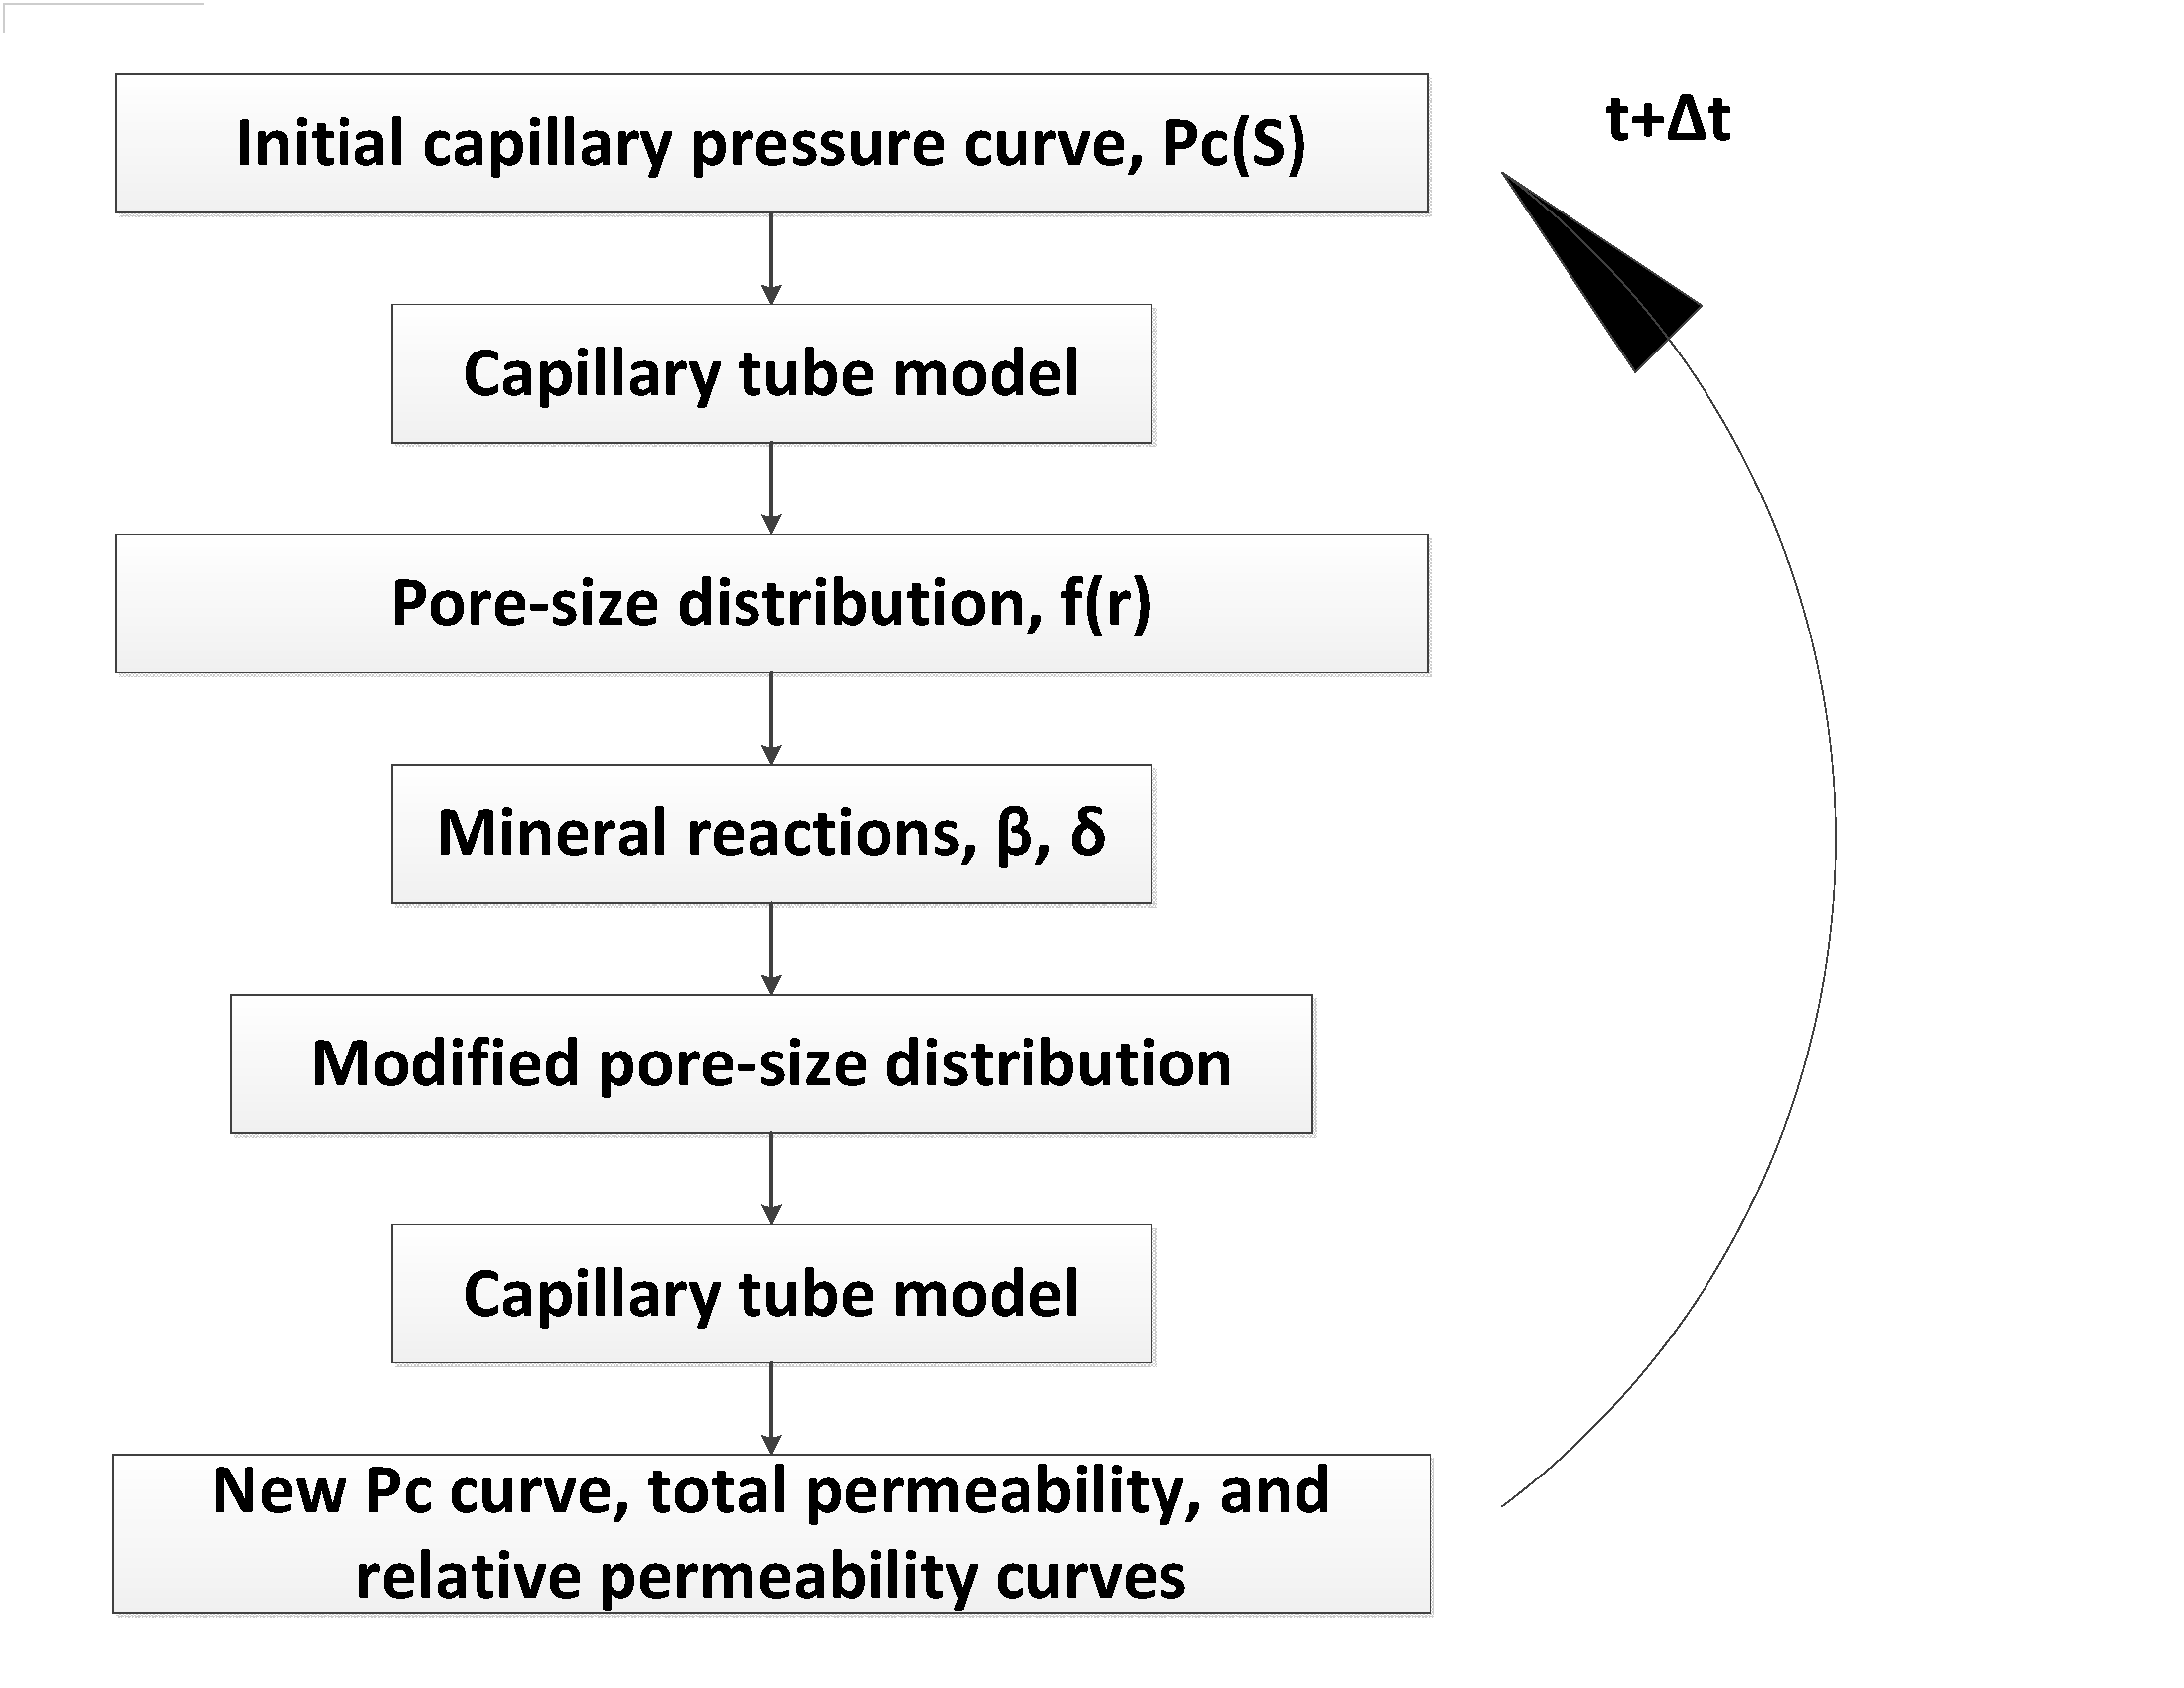
\includegraphics[width=0.8\linewidth]{PoreBundleModel.pdf}
\caption{Work flow to develop new constitute relations for multi-phase flow properties and chemical reactions.}\label{fig:workflow} 
\end{figure}


\begin{figure} 
\centering \newlength\figureheight \newlength\figurewidth\setlength\figureheight{6cm} \setlength\figurewidth{6cm} \input{example.tikz} \caption{Change of capillary pressure curve after mineral dissolution. Red dash-dot line illustrates the approach used in the precipitation case, which gives un-physical results in the dissolution case. Blue dashed line represents the correct new capillary pressure curve as discribed by Eq.\ref{eq:PcDss}. For any capillary pressure head $h$ on the new curve, its saturation S can be determined from volume balance (Eq.\ref{eq:S-S1}). } \label{fig:example} 
\end{figure}

\begin{figure}[h]
\centering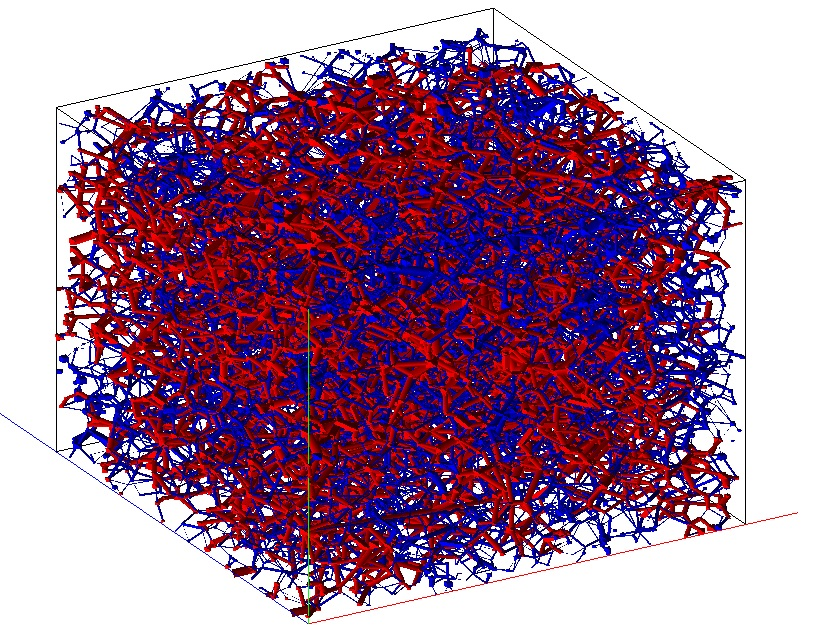
\includegraphics[width=0.8\linewidth]{PNM.jpg}
\caption{Snap shot of the Berea pore network model at water saturation of 0.5. Blue color represents water, red color represents the non-wetting phase. Size of the model is 2.14 mm x 2.14 mm x 2.14 mm.}\label{fig:PNM} 
\end{figure}


\begin{figure} 
\centering \setlength\figureheight{6cm} \setlength\figurewidth{6cm} \input{vanPc.tikz} \caption{Initial capillary pressure data from pore network modeling and fitting with van Genuchten relation.} \label{fig:vanPc} 
\end{figure}

\begin{figure} 
\centering \setlength\figureheight{6cm} \setlength\figurewidth{6cm} \input{vanKr.tikz} \caption{Initial relative permeabilities of water and non-wetting phase from pore network modeling and comparison with van Genuchten relations using parameters from \ref{fig:vanPc}.} \label{fig:vanKr} 
\end{figure}

%
\begin{figure} 
\centering  \setlength\figureheight{6cm} \setlength\figurewidth{6cm} \input{PermPoro.tikz} \caption{Permeability change as a function of porosity change predicted from current model and pore network modeling ($S_p=0.5$), compared with tranditional approach where all pores and throats are assumed to have chemical reactions ($S_p=1.0$). In our model, $S_p=0.5, \phi_0=0.24$, the value of $\beta$ ranges from 0.583 to 1.25, and the value of $\delta$ ranges from 0.088 to 2.73.} \label{fig:PermPoro} 
\end{figure}
%
%\begin{figure} 
%\centering \setlength\figureheight{6cm} \setlength\figurewidth{6cm} \input{PSD.tikz} \caption{Pore size distribution function of the Berea sandstone before precipitation and after precipitation. Porosity decreases from 0.24 to 0.22. Only pores smaller than 30 microns are affected} \label{fig:PSD} 
%\end{figure}

\begin{figure} 
\centering \setlength\figureheight{6cm} \setlength\figurewidth{6cm} \input{PcPcp.tikz} \caption{New capillary pressure curve after mineral precipitation predicted from our model and comparison with pore network modeling, using the new approach.} \label{fig:PcPcp} 
\end{figure}

\begin{figure} 
\centering \setlength\figureheight{6cm} \setlength\figurewidth{6cm} \input{KrwPcp.tikz} \caption{New water relative permeability curve after mineral precipitation predicted from our model and comparison with pore network modeling, using the new approach.} \label{fig:KrwPcp} 
\end{figure}

\begin{figure} 
\centering \setlength\figureheight{6cm} \setlength\figurewidth{6cm} \input{KrgPcp.tikz} \caption{New relative permeability of the non-wetting phase after mineral precipitation predicted from our model and comparison with pore network modeling, using the new approach.} \label{fig:KrgPcp} 
\end{figure}

\begin{figure} 
\centering \setlength\figureheight{6cm} \setlength\figurewidth{6cm} \input{PcDss.tikz} \caption{New capillary pressure curve after mineral dissolution predicted from our model and comparison with pore network modeling, using the new approach.} \label{fig:PcDss} 
\end{figure}

\begin{figure} 
\centering\setlength\figureheight{6cm} \setlength\figurewidth{6cm} \input{KrwDss.tikz} \caption{New water relative permeability curve after mineral dissolution predicted from our model and comparison with pore network modeling, using the new approach.} \label{fig:KrwDss} 
\end{figure}

\begin{figure} 
\centering \setlength\figureheight{6cm} \setlength\figurewidth{6cm} \input{KrgDss.tikz} \caption{New relative permeability curve of the non-wetting phase after mineral dissolution predicted from our model and comparison with pore network modeling, using the new approach.} \label{fig:KrgDss} 
\end{figure}
%
%\begin{figure} 
%\centering \setlength\figureheight{6cm} \setlength\figurewidth{6cm} \input{AllPcPcp.tikz} \caption{New capillary pressure curve after mineral precipitation predicted from our model and compare with pore network modeling, using the traditional approach} \label{fig:AllPcPcp} 
%\end{figure}
%
%\begin{figure} 
%\centering \setlength\figureheight{6cm} \setlength\figurewidth{6cm} \input{AllKrwPcp.tikz} \caption{New water relative permeability curve after mineral precipitation predicted from our model and compare with pore network modeling, using the traditional approach} \label{fig:AllKrwPcp} 
%\end{figure}
%
%\begin{figure} 
%\centering \setlength\figureheight{6cm} \setlength\figurewidth{6cm} \input{AllKrgPcp.tikz} \caption{New oil relative permeability after mineral precipitation predicted from our model and compare with pore network modeling, using the traditional approach} \label{fig:AllKrgPcp} 
%\end{figure}
%
%\begin{figure} 
%\centering \setlength\figureheight{6cm} \setlength\figurewidth{6cm} \input{AllPcDss.tikz} \caption{New capillary pressure curve after mineral dissolution predicted from our model and compare with pore network modeling, using the traditional approach} \label{fig:AllPcDss} 
%\end{figure}
%
%\begin{figure} 
%\centering\setlength\figureheight{6cm} \setlength\figurewidth{6cm} \input{AllKrwDss.tikz} \caption{New water relative permeability curve after mineral dissolution predicted from our model and compare with pore network modeling, using the traditional approach} \label{fig:AllKrwDss} 
%\end{figure}
%
%\begin{figure} 
%\centering \setlength\figureheight{6cm} \setlength\figurewidth{6cm} \input{AllKrgDss.tikz} \caption{New oil relative permeability curve after mineral dissolution predicted from our model and compare with pore network modeling, using the traditional approach} \label{fig:AllKrgDss} 
%\end{figure}
%



\end{document}

%%
%% End of file `elsarticle-template-1-num.tex'.
